\iffalse
\section{Illustration of the Morse-Smale Complex}
\label{app:example}

% \begin{figure}[h]
%  \centering
%  %\resizebox{0.9\columnwidth}{!}{%
%  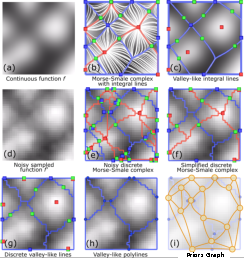
\includegraphics[width=0.6\textwidth]{./figures/mscbackground.pdf}
%  %}
%      \caption{ Morse-Smale complexes are defined for functions with continuous gradients {\bf(a-c)}. A smooth function {\bf(a)} can be partitioned based on the behavior of integral lines {\bf(b)}, with selected integral lines shown in white. This partition forms a cell complex, where integral lines within each cell share a common origin and destination. The 0-dimensional cells are  maxima (red), saddles (green), and minima (dark blue)), the 1-dimensional cells are formed by ascending (orange) and descending lines (light blue) from saddles (green), and 2-dimensional cells are bounded by 0- and 1-cells {\bf(b)}. Elements of this complex often form semantic features of interest in a scientific domain, such as valley-like lines {\bf(c)}. Real-world functions often come from noisy sources, and are available as samples on a grid {\bf(d)}. Discrete Morse-theory-based methods allow practical computation of Morse-Smale complexes {\bf(e)}, which encode both noise and discretization artifacts that may be simplified to recover the coarse-scale behavior of the function {\bf(f)}. The valley-like structures may be extracted from this complex {\bf(g)}, and converted to a set of priors between non-degree-2 vertices denoted the valley graph {\bf(h)}. The priors graph (yellow), {\bf(i)}, represents each prior as a vertex with edges between incident priors. }
%      \label{mscbackground}
%  \end{figure}
\fi
 



